\documentclass[aspectratio=169]{beamer}
\usetheme{metropolis}
\usepackage{appendixnumberbeamer}

\usepackage{booktabs}
\usepackage[scale=2]{ccicons}

\usepackage{graphicx}
\usepackage{pgfpages}

\usepackage{xspace}
\newcommand{\themename}{\textbf{\textsc{metropolis}}\xspace}

%Information to be included in the title page:
\title{Public Key Infrastructure (PKI)}
\subtitle{Introduction}
\author{Ritger Teunissen (ritger@hack42.nl)}
\institute{Hack42, Arnhem}
\date{\today}
%\setbeameroption{show notes on second screen=right}

%\usebackgroundtemplate
%{
%    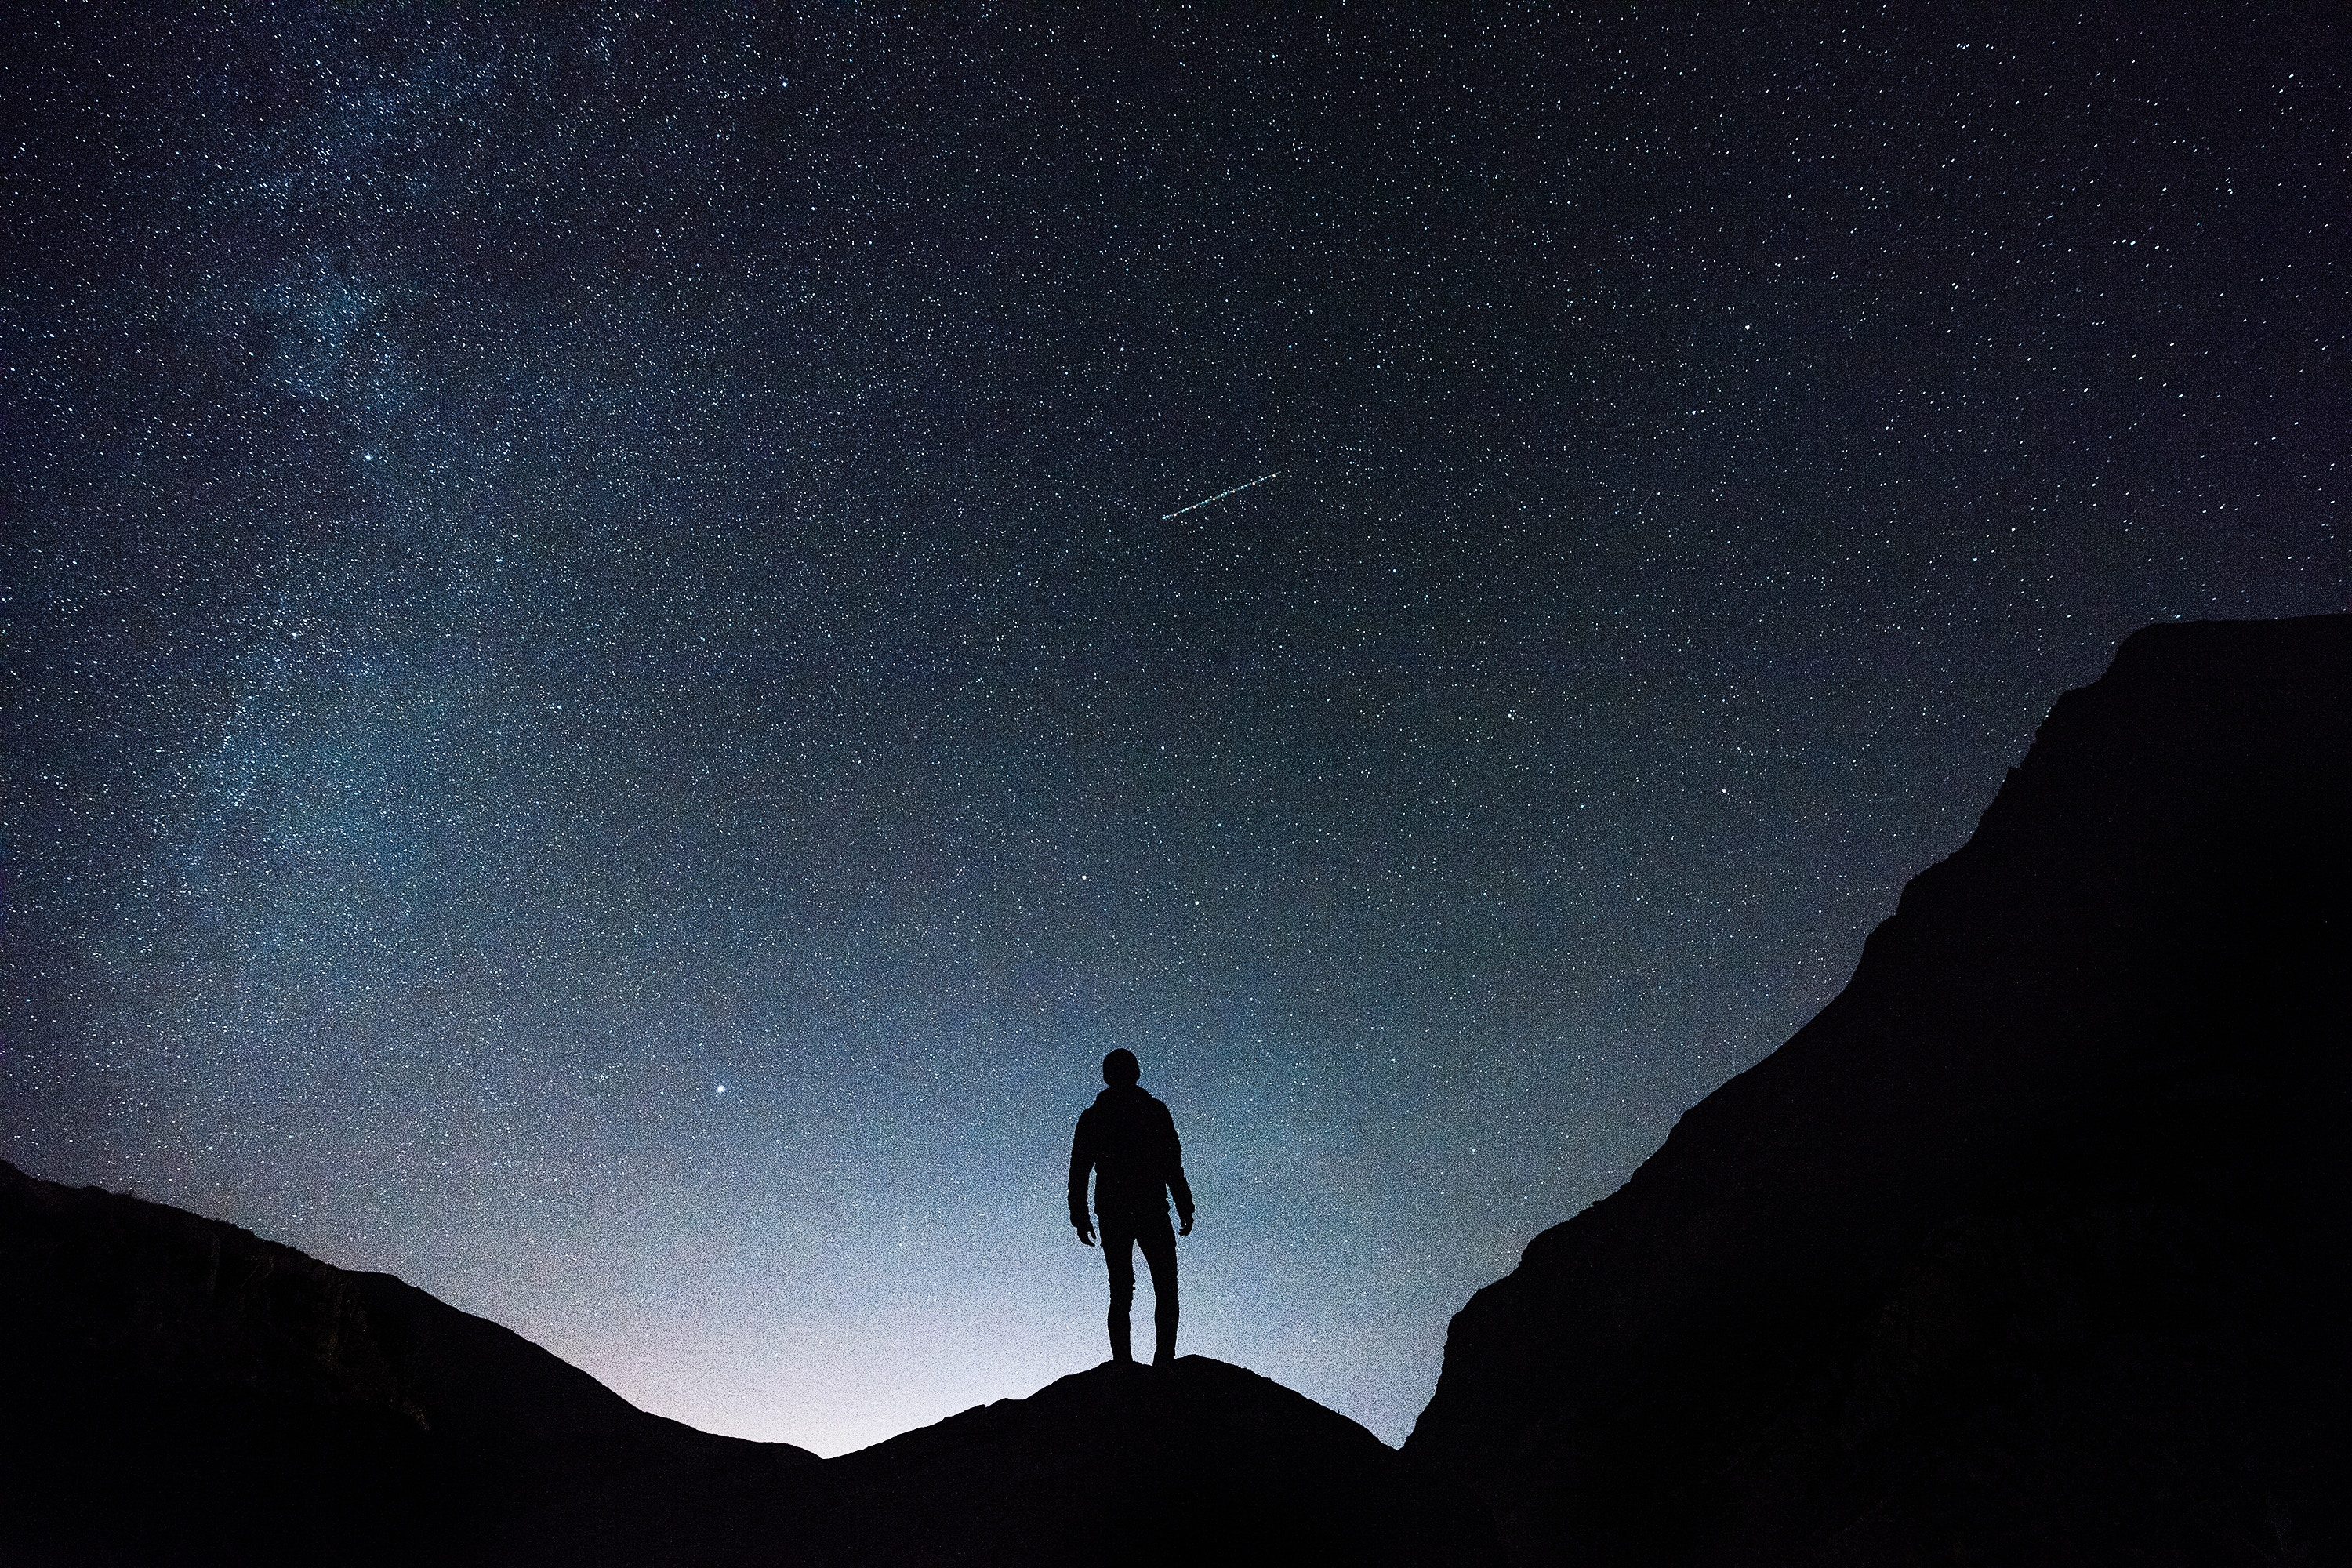
\includegraphics[width=\paperwidth,height=\paperheight]{images/background.jpg}
%}

% TODO: Add transition sentence to next slide for each slide

\begin{document}
    \maketitle
    \begin{frame}{Who am I?}
        \begin{itemize}
            \item Worked in Information Security for 12 years
            \item \emph{Member} of \alert{Hack42} (https://www.hack42.nl/)
        \end{itemize}
        \note[item]{Worked in Information Security for 12 years}
        \note[item]{Member of Hack42 (https://www.hack42.nl)}
    \end{frame}

%    {
%    \usebackgroundtemplate{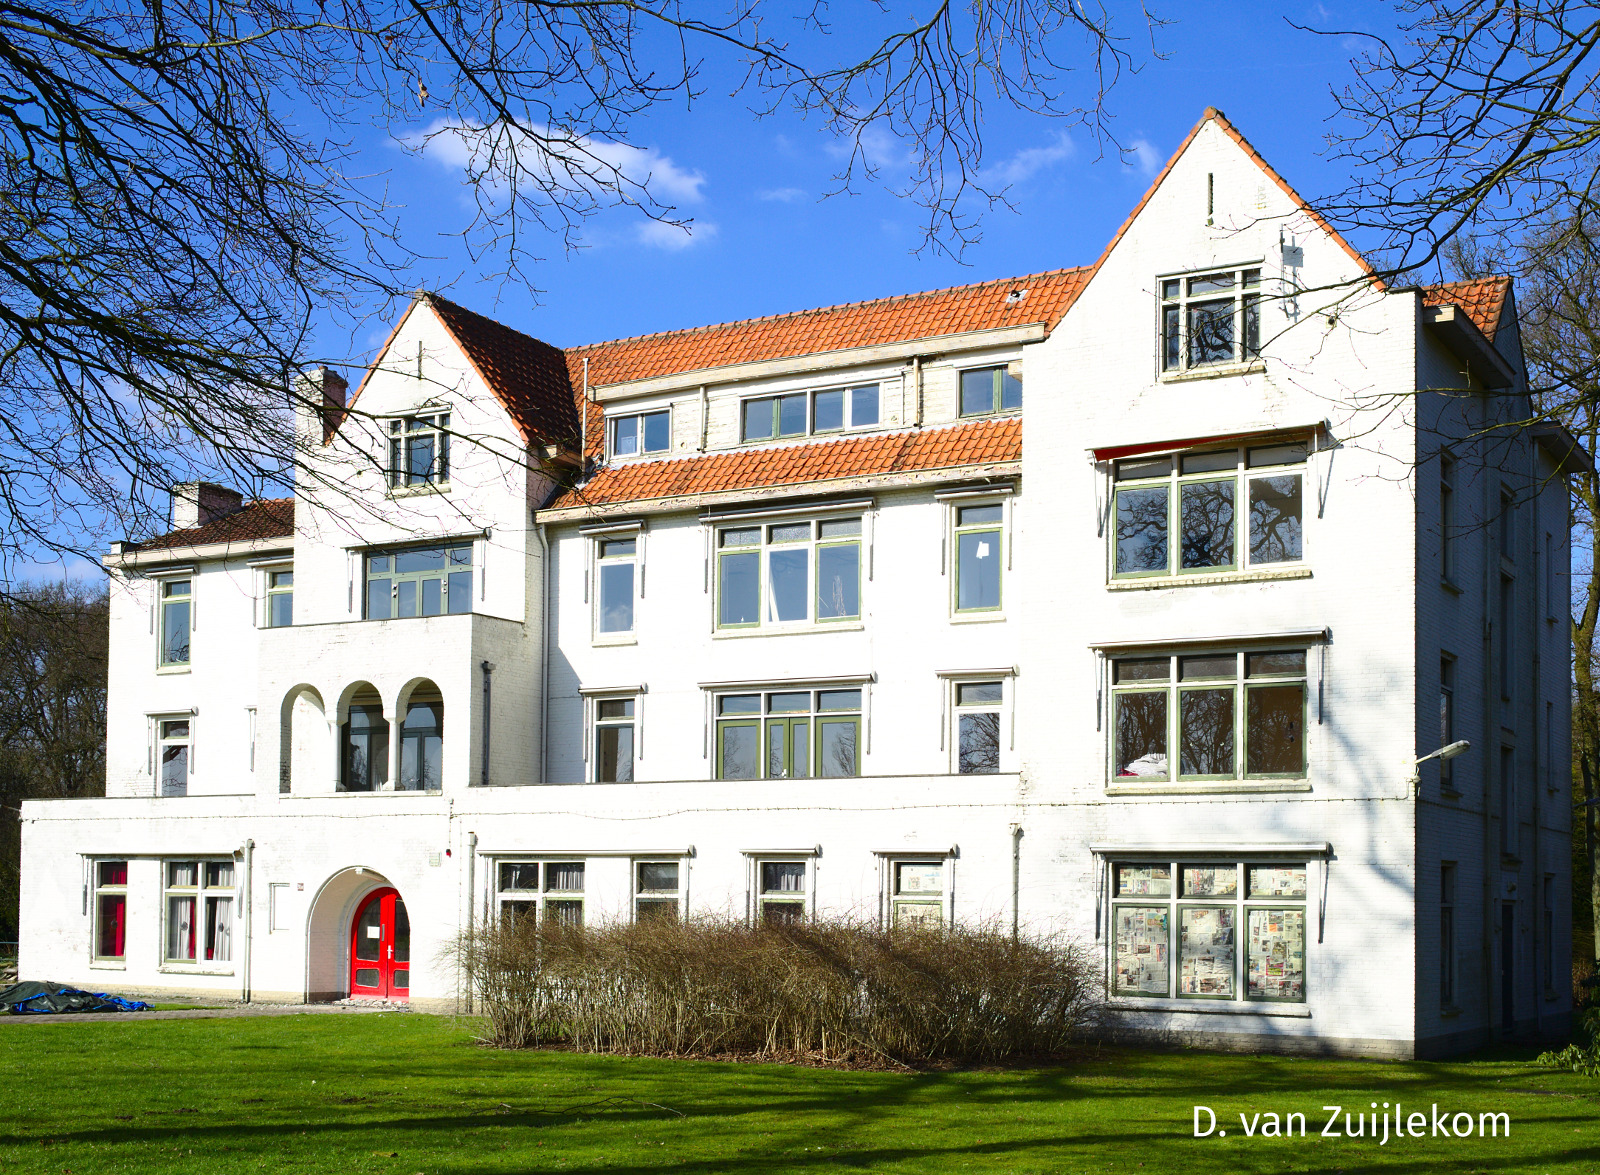
\includegraphics[height=\paperheight]{images/vrijland.jpg}}%
%    \begin{frame}{Hack42 - Vrijland}
%    \end{frame}
%    }
%
%    {
%    \usebackgroundtemplate{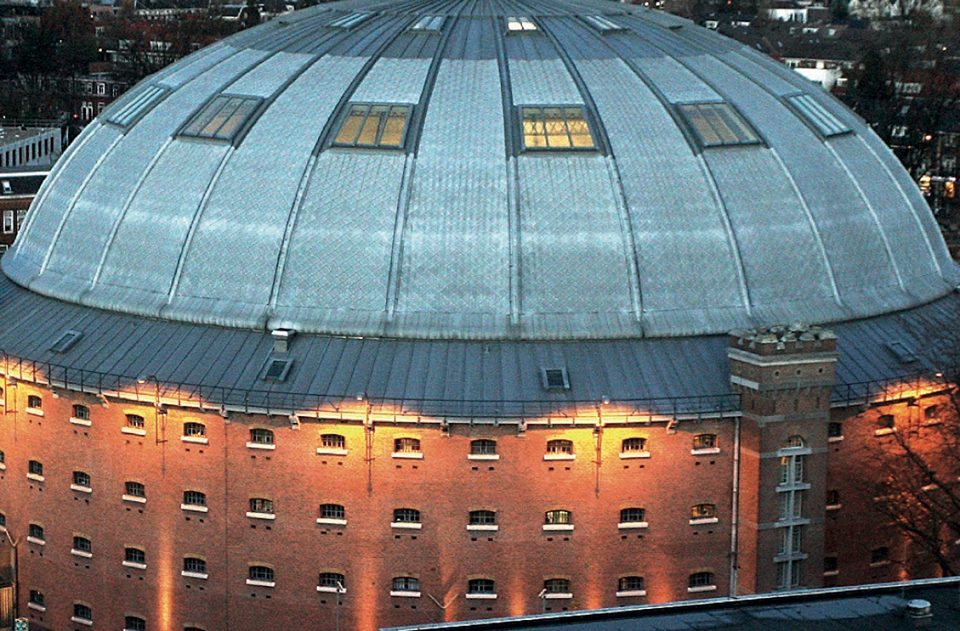
\includegraphics[height=\paperheight]{images/koepelgevangenis.jpg}}%
%    \begin{frame}{Bee Hive 4.2 (https://beehive42.org/)}
%    \end{frame}
%    }

    \begin{frame}{Table of Contents}
        \setbeamertemplate{section in toc}[sections numbered]
        \tableofcontents[hideallsubsections]
    \end{frame}

    \section{Background}

    \begin{frame}{What is PKI?}
        \begin{quote}
            \centering
            PKI is a (supporting) technical solution used to secure \alert{digital communication}
        \end{quote}
        \note[item]{PKI is a (supporting) technical solution used to secure \alert{digital communication}}
        \note[item]{Abstract definition, lets see some examples first}
    \end{frame}

    \begin{frame}{Real-life Examples}
        \begin{figure}[h]
            \centering
            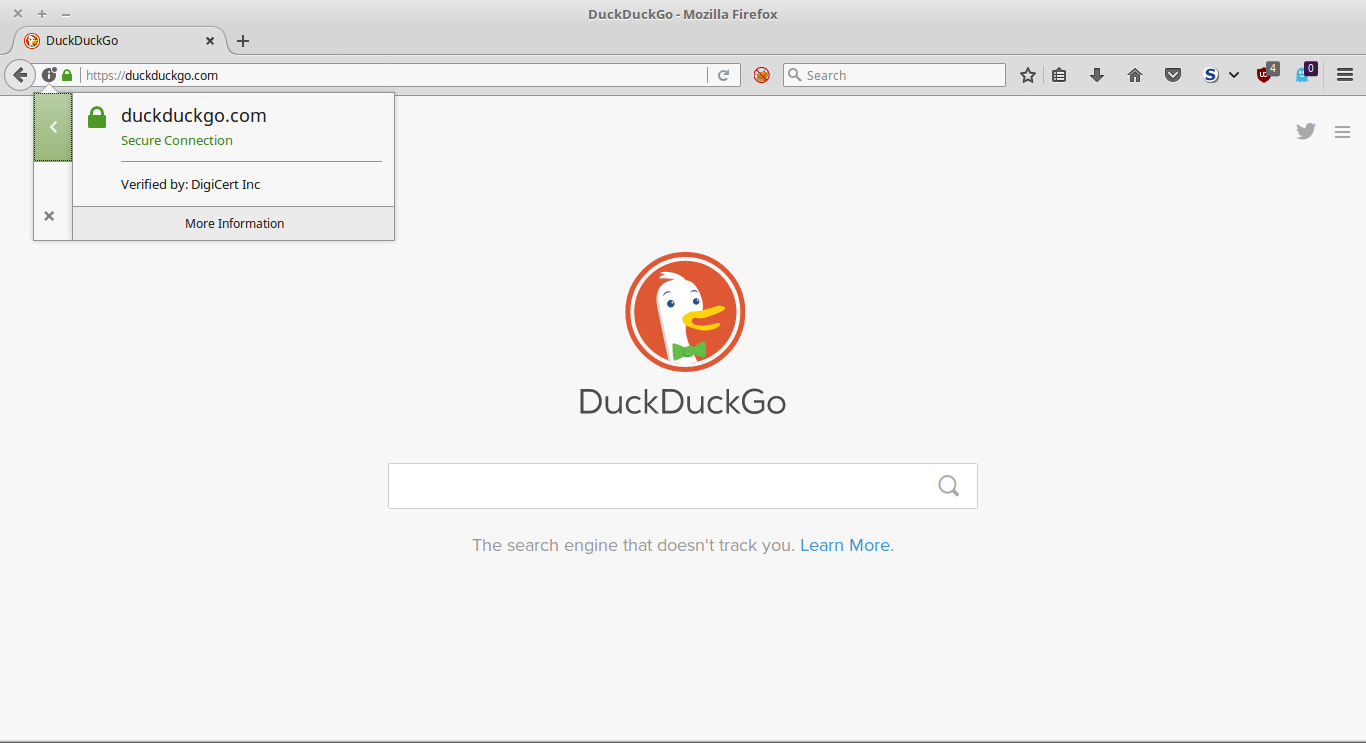
\includegraphics[width=300pt,keepaspectratio]{images/duck_duck_go.png}
            \caption{Duck Duck Go}
        \end{figure}
        \note[item]{Am I really visiting the correct website?}
    \end{frame}

    \begin{frame}{Real-life Examples}
        \begin{figure}[h]
            \centering
            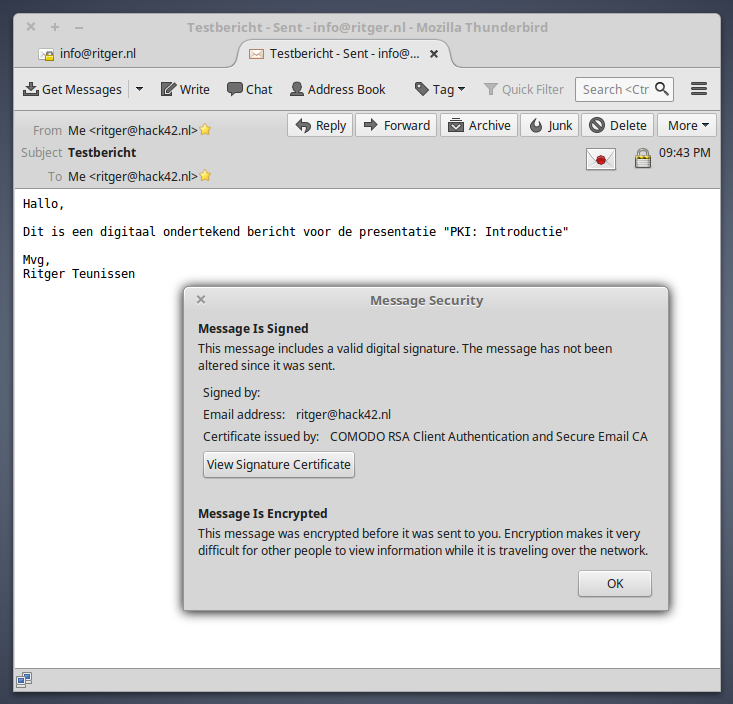
\includegraphics[width=180pt,keepaspectratio]{images/thunderbird.png}
            \caption{E-mail}
        \end{figure}
        \note[item]{Is this e-mail really written by me and can only the receiver and I read it?}
    \end{frame}

    % @TODO: Why should you care?

    \begin{frame}{Communication}
        \begin{figure}[h]
            \centering
            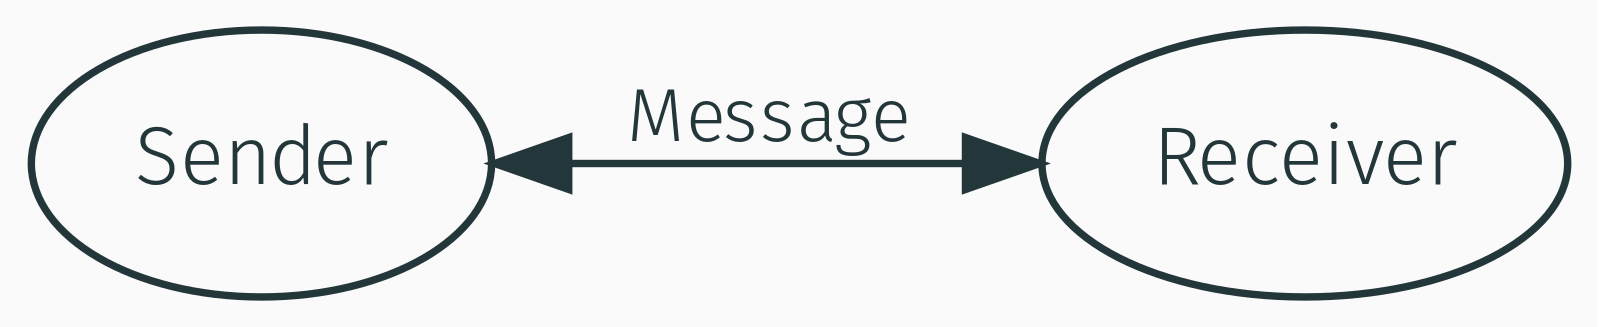
\includegraphics[width=300pt,keepaspectratio]{images/communication.png}
            \caption{Communication}
        \end{figure}
        \note[item]{Both examples are communication: between you and a website, between you and the e-mail receiver}
        \note[item]{Communication - Sender/receiver/messages}
        \note[item]{Everything we do on the internet is based on digital communication}
    \end{frame}

    \begin{frame}{Securing Digital Communication}
        \begin{quote}
            \centering
            When can \alert{digital communication} be considered secure?
        \end{quote}
        \pause
        \begin{exampleblock}{Authenticity}
            Do we know who the sender is?
        \end{exampleblock}
        \pause
        \begin{exampleblock}{Non-repudiation}
            Did the message really come from the sender and hasn't the message been changed?
        \end{exampleblock}
        \pause
        \begin{exampleblock}{Confidentiality}
            Can the message only be read by the sender and receiver?
        \end{exampleblock}
        \note[item]{Authenticity: Do we know who the sender is?}
        \note[item]{Non-repudiation: Did the message really come from the sender and hasn't the message been changed?}
        \note[item]{Confidentiality: Can the message only be read by the sender and receiver?}
        \note[item]{I have nothing to hide, so you don't have to look}
        \note[item]{So how do we keep our communication secure?}
    \end{frame}

    \section{Asymmetric Cryptography}

    \begin{frame}{Cryptography}
        \begin{quote}
            \centering When you use cryptography to solve a problem, you have \alert{\sc{two}} problems
        \end{quote}
        \note[item]{When you use cryptography to solve a problem, you have two problems}
        \note[item]{Lets start with what we need to do asymmetric cryptography}
    \end{frame}

    \begin{frame}{Asymmetric Cryptography}
        \begin{figure}[h]
            \centering
            \includegraphics<1>[width=300pt,keepaspectratio]{images/gen_key_pair_01.png}
            \includegraphics<2>[width=300pt,keepaspectratio]{images/gen_key_pair_02.png}
            \caption{Key Generation}
        \end{figure}
        \pause
        \begin{exampleblock}{Key Pair}
            A key pair has both a public and private key
        \end{exampleblock}
        \note[item]{Key pair has both a public and private key}
        \note[item]{Public and private key are mathematically related}
        \note[item]{Private key is kept secret (very important!), public key is distributed}
        \note[item]{Trust is established by exchanging public keys}
    \end{frame}

    \begin{frame}{Non-repudiation}
        \begin{figure}[h]
            \centering
            \includegraphics<1>[width=300pt,keepaspectratio]{images/sign_01.png}
            \includegraphics<2>[width=300pt,keepaspectratio]{images/sign_02.png}
            \includegraphics<3>[width=300pt,keepaspectratio]{images/sign_03.png}
            \caption{Digital Signature}
        \end{figure}
        \note[item]{A digital signature becomes invalid if the message is changed}
    \end{frame}

    \begin{frame}{Non-repudiation}
        \begin{exampleblock}{Example}
            Digitally signing a document or e-mail message
        \end{exampleblock}
    \end{frame}

    \begin{frame}{Confidentiality}
        \begin{figure}[h]
            \centering
            \includegraphics<1>[width=300pt,keepaspectratio]{images/encrypt_01.png}
            \includegraphics<2>[width=300pt,keepaspectratio]{images/encrypt_02.png}
            \includegraphics<3>[width=300pt,keepaspectratio]{images/encrypt_03.png}
            \caption{Encryption}
        \end{figure}
        \pause
        \note[item]{The message is encrypted using the public key of the recipient}
        \note[item]{The message is decrypted using the private key of the recipient}
    \end{frame}

    \begin{frame}{Confidentiality}
        \begin{exampleblock}{Example}
            Encrypting a document or e-mail message
        \end{exampleblock}
    \end{frame}

    \begin{frame}{Authenticity}
        \begin{exampleblock}{How to prove authenticity?}
            Prove possession of the private key for a public key
        \end{exampleblock}
        \begin{figure}[h]
            \centering
            \includegraphics<1>[width=300pt,keepaspectratio]{images/auth_01.png}
            \includegraphics<2>[width=300pt,keepaspectratio]{images/auth_02.png}
            \includegraphics<3>[width=300pt,keepaspectratio]{images/auth_03.png}
            \includegraphics<4>[width=300pt,keepaspectratio]{images/auth_04.png}
            \caption{Authenticity}
        \end{figure}
        \pause
        \note[item]{This is the first example, visiting a website}
        \note[item]{Possession of the private key belonging to the public key proves that you are who you say you are}
        \note[item]{Says nothing about the content being sent!}
        \note[item]{Only that Bob has the private key belonging to the public key}
    \end{frame}

    \begin{frame}{Authenticity}
        \begin{quote}
            \centering
            Why is authenticity separate from non-repudiation?
        \end{quote}
        \pause
        \begin{exampleblock}{Answer}
            Prevent \alert{unintended} signature creation
        \end{exampleblock}
        \note[item]{Technically the same}
        \note[item]{Two separate functional use cases}
        \note[item]{Conclusion: every use case requires its own key pair}
    \end{frame}

    \begin{frame}{Summary}
        \begin{quote}
            \centering
            What do you \alert{need} to know?
        \end{quote}
        \pause
        \begin{alertblock}{Key Pair}
            Both a public and private key. \emph{All} users need to have \emph{all} public keys
        \end{alertblock}
        \pause
        \begin{alertblock}{Digital Signature}
            Sign using the private key, verify using the public key
        \end{alertblock}
        \pause
        \begin{alertblock}{Encryption}
            Encryption using the public key, decryption using the private key
        \end{alertblock}
        \note[item]{Key Pair: Both a public and private key. \emph{All} users need to have \emph{all} public keys}
        \note[item]{Digital Signature: Sign using the private key, verify using the public key}
        \note[item]{Encryption: Encryption using the public key, decryption using the private key}
    \end{frame}

    \section{Public Key Infrastructure}

    \begin{frame}{Key Distribution}
        \begin{figure}[h]
            \centering
            \includegraphics[width=200pt,keepaspectratio]{images/public_keys.png}
            \caption{Key Distribution}
        \end{figure}
        \note[item]{Everybody needs to have everybody's public key}
        \note[item]{PKI provides a solution for the key distribution problem}
        \note[item]{Public keys need to be distributed out-of-band}
        \note[item]{Accepting a public key = trusting owner of related private key}
        \note[item]{Key distribution does not scale}
    \end{frame}

    \begin{frame}{Delegated Trust}
       \begin{figure}[h]
           \centering
           \includegraphics[width=170pt,keepaspectratio]{images/pki.png}
           \caption{Delegated Trust}
       \end{figure}
        \note[item]{PKI provides delegation of individual trust}
        \note[item]{Users do not trust eachother directly, but trust a single party}
        \note[item]{Users only need the public from this single party}
        \note[item]{Single party = CA}
    \end{frame}

    \begin{frame}{Certificate Authority (1)}
        \begin{quote}
            \centering
            What is a Certificate Authority?
        \end{quote}
        \pause
        \begin{itemize}
            \item Certifies the link between an identity and a public key
            \pause
            \item Certifies a key for specific use cases
            \pause
            \item Can revoke trust in a public key
        \end{itemize}
        \note[item]{Certifies the link between an identity and a public key}
        \note[item]{Certifies a key for specific applications}
        \note[item]{Can revoke trust in a public key}
    \end{frame}

    \begin{frame}{X.509 Certificates}
        \begin{columns}[T,onlytextwidth]
            \column{0.5\textwidth}
                \begin{figure}[h]
                    \centering
                    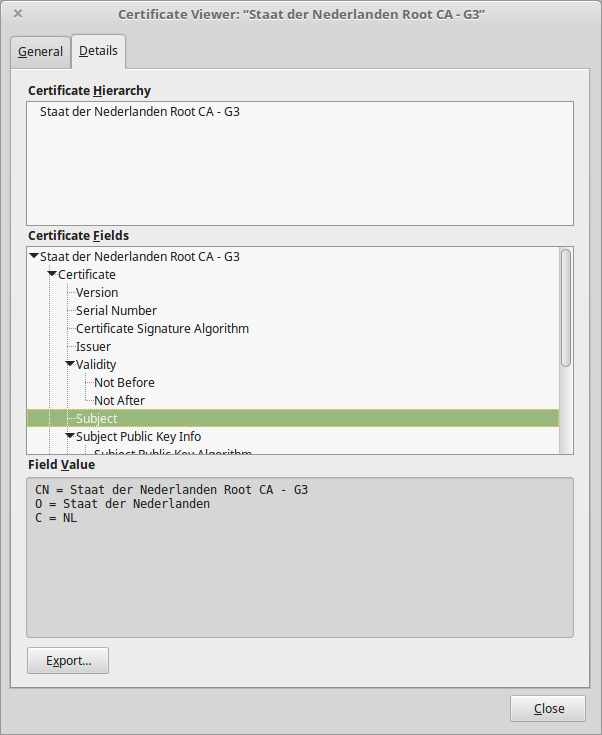
\includegraphics[width=110pt,keepaspectratio]{images/staat_der_nederlanden_root_ca.png}
                    \caption{X.509 Certificate}
                \end{figure}
            \column{0.5\textwidth}
                \begin{itemize}
                    \pause
                    \item Certificate = identity + public key
                    %\pause
                    \item Limits key usage
                    %\pause
                    \item Limited validity (best-before date)
                    %\pause
                    \item Certificate Revocation List
                    %\pause
                    \item \alert{Digitally signed by issuer (CA)}
                \end{itemize}
        \end{columns}
        \note[item]{Certificate = identity + public key}
        \note[item]{Limits key usage}
        \note[item]{Limited validity (best-before date)}
        \note[item]{Certificate Revocation List}
        \note[item]{\alert{Digitally signed by issuer (CA)}}
    \end{frame}

    \begin{frame}{Certificate Authority (2)}
        \begin{itemize}
            \item Generates its own key pair (public and private key)
            \pause
            \item Issues its own X.509 \alert{CA} certificate
            \pause
            \item Issues X.509 certificates for end entities
            \pause
            \item Makes X.509 certificate non-reputable through a digital signature
        \end{itemize}
        \note[item]{Generates its own key pair (public and private key)}
        \note[item]{Issues its own X.509 \alert{CA} certificate}
        \note[item]{Issues X.509 certificates for end entities}
        \note[item]{Makes X.509 certificate non-reputable through a digital signature}
    \end{frame}

    \begin{frame}{Setup}
        \begin{figure}[h]
            \centering
            \includegraphics<1>[width=300pt,keepaspectratio]{images/ca_01.png}
            \includegraphics<2>[width=300pt,keepaspectratio]{images/ca_02.png}
            \includegraphics<3>[width=300pt,keepaspectratio]{images/ca_03.png}
            \caption{PKI Architecture}
        \end{figure}
        \note[item]{Root CA}
        \note[item]{Intermediate CA}
        \note[item]{End entity = identity}
    \end{frame}

    \begin{frame}{CA Trust}
        \begin{quote}
            \centering
            How is a (CA) certificate trusted?
        \end{quote}
        \pause
        \begin{exampleblock}{End-entity \& Intermediate CA}
            Trusted when the digital signature created by the CA is valid and the certificate has not been revoked
        \end{exampleblock}
        \pause
        \begin{exampleblock}{Root CA}
            Trusted through the use of an Access Control List
        \end{exampleblock}
        \note[item]{How is a (CA) certificate trusted?}
        \note[item]{End-entity \& Intermediate CA: Trusted when the digital signature created by the CA is valid and the certificate has not been revoked}
        \note[item]{Root CA: Trusted through the use of an Access Control List}
    \end{frame}

    \begin{frame}{Largest Use Case}
        \begin{quote}
            \centering
            Prove authenticity of devices
        \end{quote}
        \pause
        \begin{exampleblock}{Web Server}
            Is issued an end entity certificate by a CA, which allows clients to trust the web server by its address (FQDN)
        \end{exampleblock}
        \note[item]{Web Server: Is issued an end entity certificate by a CA, which allows clients to trust the web server by its identity: web address (FQDN)}
        \note[item]{Only the web server has the private key for the X.509 certificate, see Authentication (Asymmetric Cryptography)}
    \end{frame}

    \begin{frame}{Public \& Private Trust}
        \begin{itemize}
            \item Private CAs issue X.509 certificates for a closed (usually corporate) environment
            \pause
            \item Publicly trusted CAs issue X.509 certificates which are \alert{automatically} trusted
        \end{itemize}
        \note[item]{Trust stores contain Root CA certificates in mobile devices, OS}
        \note[item]{Private CAs issue X.509 certificates for a closed (usually corporate) environment}
        \note[item]{Publicly trusted CAs issue X.509 certificates which are \alert{automatically} trusted}
    \end{frame}

    \begin{frame}{CA/B Forum}
        \begin{figure}[h]
            \centering
            \includegraphics[width=330pt,keepaspectratio]{images/logos.png}
            \caption{CA/B Forum}
        \end{figure}
        \note[item]{Two major players: Browsers \& CA's}
        \note[item]{Power concentrated with the Browsers, they implement the trust stores}
    \end{frame}

    \begin{frame}{Problem?}
        \begin{quote}
            \centering
            What could possibly go wrong?
        \end{quote}
        \note[item]{What if something goes wrong?}
    \end{frame}

    {
    \usebackgroundtemplate{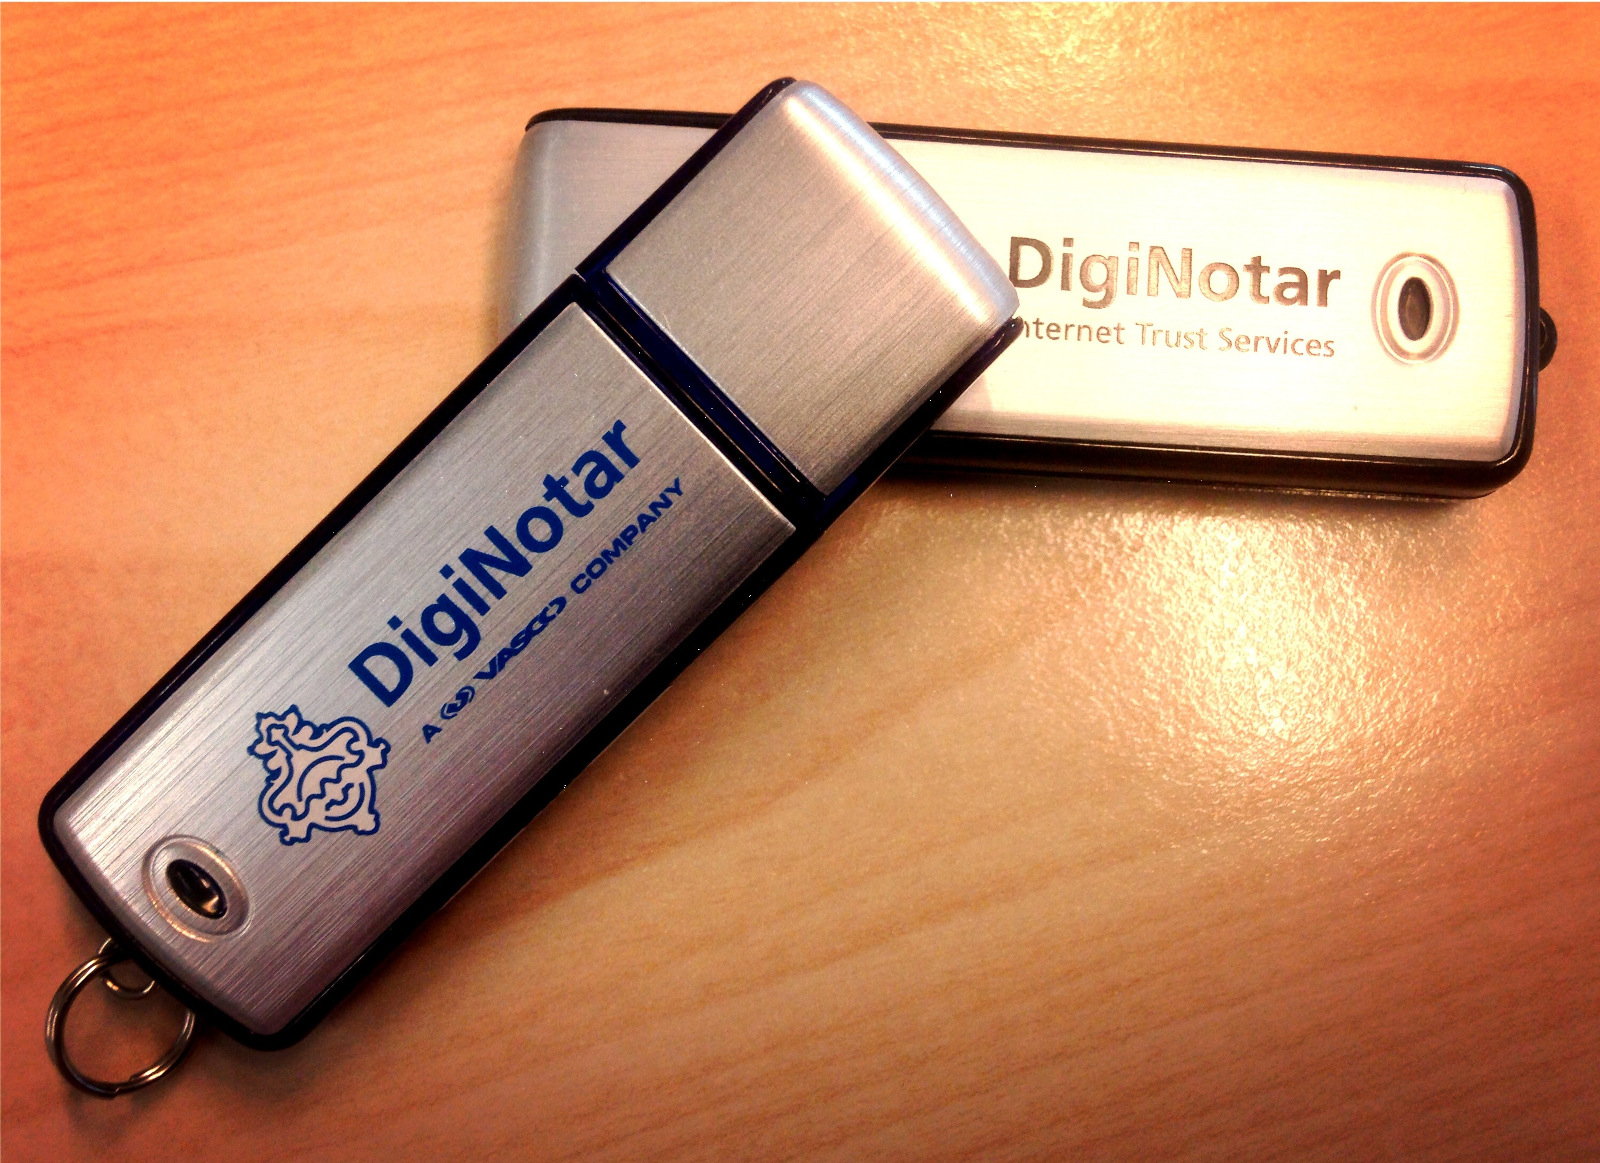
\includegraphics[width=\paperwidth]{images/diginotar.jpg}}%
    \begin{frame}{DigiNotar}
        \note[item]{Compromise public in September 2011, bankrupt in October}
        \note[item]{Suplier of 60\% of all government X.509 certificates, including Tax Office}
        \note[item]{Extreme audit failure: E\&Y, Vasco, OPTA}
        \note[item]{Should have been revoked immediately, did not happen}
        \note[item]{X.509 certificates needed to be replaced first}
    \end{frame}
    }

    \begin{frame}{Summary}
        \begin{quote}
            \centering
            What do you \alert{need} to know?
        \end{quote}
        \pause
        \begin{alertblock}{Key Distribution}
            Key distribution is a difficult problem to solve at scale
        \end{alertblock}
        \pause
        \begin{alertblock}{Delegated Trust}
            Key distribution is much easier when trust is centralised
        \end{alertblock}
        \pause
        \begin{alertblock}{Certificate Authority}
            In PKI, the Certificate Authority manages trust. Everything start (or stops) with the CA
        \end{alertblock}
        \note[item]{Key distribution: difficult problem to solve at scale}
        \note[item]{Delegated Trust: Key distribution is much easier when trust is centralised}
        \note[item]{Certificate Authority: In PKI, the Certificate Authority manages trust. Everything start (or stops) with the CA}
    \end{frame}

    \begin{frame}{Conclusion}
        \begin{itemize}
            \item A \alert{key pair} (public and private key) is used to secure digital communication.
            \pause
            \item Trust is delegated to a \alert{Certificate Authority} (CA)
            \pause
            \item Certificate Authorities certify the combination of
                identity + key (including the CA public key itself)
            \pause
            \item Global trust is managed by a small group of (very powerful)
                companies (\alert{CA/B Forum})
        \end{itemize}
        \note[item]{A \alert{key pair} (public and private key) is used to secure digital communication.}
        \note[item]{Trust is delegated to a \alert{Certificate Authority} (CA)}
        \note[item]{Certificate Authorities certify the combination of identity + key (including the CA public key itself)}
        \note[item]{Global trust is managed by a small group of (very powerful) companies (\alert{CA/B Forum})}
    \end{frame}

    \begin{frame}[standout]
        Questions?
    \end{frame}

    \section{Certificate Life Cycle}

    \begin{frame}{Certificate Life Cycle}
        \begin{figure}[h]
            \centering
            \includegraphics<1>[width=300pt,keepaspectratio]{images/life_cycle_01.png}
            \includegraphics<2>[width=300pt,keepaspectratio]{images/life_cycle_02.png}
            \includegraphics<3>[width=300pt,keepaspectratio]{images/life_cycle_03.png}
            \includegraphics<4>[width=300pt,keepaspectratio]{images/life_cycle_04.png}
            \includegraphics<5>[width=300pt,keepaspectratio]{images/life_cycle_05.png}
            \includegraphics<6>[width=300pt,keepaspectratio]{images/life_cycle_06.png}
            \caption{Certificate Life Cycle}
        \end{figure}
        \note[item]{Registration}
        \note[item]{Attestation}
        \note[item]{Issuance}
        \note[item]{Management}
        \note[item]{Revocation}
    \end{frame}

    \begin{frame}{Certificate Life Cycle}
        \begin{columns}[T,onlytextwidth]
            \column{0.5\textwidth}
            \begin{exampleblock}{Registration}
                Create a new certificate request
            \end{exampleblock}
            \begin{exampleblock}{Attestation}
                Attestation (validation) of the \\ certificate request
            \end{exampleblock}
            \begin{exampleblock}{Issuance}
                Issuance of an X.509 certificate
            \end{exampleblock}
            \column{0.5\textwidth}
            \begin{exampleblock}{Management}
                Management of issued X.509 certificates
            \end{exampleblock}
            \begin{exampleblock}{Revocation}
                Revocation of issued X.509 certificates
            \end{exampleblock}
        \end{columns}
    \end{frame}

    \begin{frame}{Challenges}
        \begin{itemize}
            \item Often forgotten or neglected
            \pause
            \item "Bob" manages certificates using \alert{Excel}
            \pause
            \item Manual work, does not scale and is expensive
        \end{itemize}
        \note[item]{Often forgotten or neglected}
        \note[item]{"Bob" manages certificates using \alert{Excel}}
        \note[item]{Manual work, does not scale and is expensive}
    \end{frame}

    \begin{frame}{Solution?}
        \begin{itemize}
            \item Automation!
            \pause
            \item Certificate Management System (CMS)
            \pause
            \item Provisioning Agents
        \end{itemize}
        \note[item]{Automation!}
        \note[item]{Certificate Management System (CMS)}
        \note[item]{Provisioning Agents}
    \end{frame}

    \begin{frame}[standout]
        Questions?
    \end{frame}
\end{document}
